\documentclass[aspectratio=169]{beamer}
\usetheme{Madrid}
\usecolortheme{default}

\usepackage{booktabs}
\usepackage{tikz}
\usepackage{xcolor}
\usepackage{amssymb}

\definecolor{goodgreen}{RGB}{34,139,34}
\definecolor{badred}{RGB}{200,30,30}
\definecolor{warnambr}{RGB}{200,150,0}

\title{Referee Report --- Round 6}
\subtitle{Tennis Match Simulator}
\date{2026-02-10}
\author{Referee 2}

\begin{document}

% ================================================================
% SLIDE 1: Title
% ================================================================
\begin{frame}
\titlepage
\end{frame}

% ================================================================
% SLIDE 2: Executive Summary
% ================================================================
\begin{frame}[t]{Data Leakage Fixed; Elo Underperformance Correctly Diagnosed}
\textbf{Verdict: Accept with Minor Revisions}

\vspace{0.8em}
\begin{itemize}
  \item \textcolor{goodgreen}{\checkmark} \textbf{Data leakage eliminated} --- date alignment module correctly resolves \texttt{tourney\_date} mismatch (89.6\% actual dates, 10.4\% inferred)
  \item \textcolor{goodgreen}{\checkmark} \textbf{Corrected results are trustworthy} --- Elo 60.8\%, MC 56.0\%, gap 4.8pp (not 9.9pp)
  \item \textcolor{goodgreen}{\checkmark} \textbf{Root cause identified} --- career trajectory lag explains systematic Elo errors
  \item \textcolor{warnambr}{$\triangle$} \textbf{Calibration and K-factor tests still pending} (flagged Rounds 3--5)
  \item \textcolor{warnambr}{$\triangle$} \textbf{Proposed fixes are untested} --- five remedies listed, zero evaluated
\end{itemize}
\end{frame}

% ================================================================
% SLIDE 3: Leakage Fix Verification
% ================================================================
\begin{frame}[t]{Leakage Fix: Date Alignment Module Works Correctly}

\begin{columns}[T]
\column{0.52\textwidth}
\textbf{How it works:} Join ATP matches with betting data on player names + tournament to inherit actual dates. Infer dates from round for unmatched events.

\vspace{0.3em}
\begin{table}
\centering
\footnotesize
\begin{tabular}{lrr}
\toprule
Strategy & N & \% \\
\midrule
Exact name match & 1,222 & 71.6\% \\
Name variants & 307 & 18.0\% \\
Inferred from round & 177 & 10.4\% \\
\midrule
\textbf{Total} & \textbf{1,706} & \textbf{100\%} \\
\bottomrule
\end{tabular}
\end{table}

\column{0.45\textwidth}
\textbf{Defensive measures:}
\begin{itemize}
  \item[\textcolor{goodgreen}{\checkmark}] Cache-first loading
  \item[\textcolor{goodgreen}{\checkmark}] Runtime fallback
  \item[\textcolor{goodgreen}{\checkmark}] Warning if no alignment
  \item[\textcolor{goodgreen}{\checkmark}] Validation function
  \item[\textcolor{goodgreen}{\checkmark}] 8 unit tests
\end{itemize}

\textbf{Residual risk:} Inferred dates (10.4\%) are for United Cup, Davis Cup --- no impact on predictions.
\end{columns}
\end{frame}

% ================================================================
% SLIDE 4: Leakage Impact Quantified
% ================================================================
\begin{frame}[t]{Leakage Inflated Elo by 7.8pp, MC by 2.7pp --- As Predicted}

\begin{columns}[T]
\column{0.50\textwidth}
\begin{table}
\centering
\begin{tabular}{lccc}
\toprule
Model & Old & Clean & Drop \\
\midrule
\textbf{Elo} & 68.6\% & \textbf{60.8\%} & \textcolor{badred}{--7.8pp} \\
MC & 58.7\% & 56.0\% & \textcolor{badred}{--2.7pp} \\
\midrule
Gap & +9.9pp & +4.8pp & \\
\bottomrule
\end{tabular}
\end{table}

\vspace{0.8em}
\begin{table}
\centering
\footnotesize
\begin{tabular}{lcc}
\toprule
Metric & Elo & MC \\
\midrule
Accuracy & 60.8\% & 56.0\% \\
Brier & 0.2331 & 0.2451 \\
Log Loss & 0.6585 & 0.6846 \\
\bottomrule
\end{tabular}
\end{table}

\column{0.47\textwidth}
\textbf{Key takeaways:}

\begin{enumerate}
  \item Elo still outperforms MC, but gap is 4.8pp not 9.9pp
  \item Leakage affected Elo 3$\times$ more than MC (as referee predicted in Round 5)
  \item \textbf{Neither model beats the market} ($\sim$67\% favorite accuracy)
  \item ROI is negative at all thresholds
\end{enumerate}

\vspace{0.5em}
\textbf{Why Elo was more affected:}\\
K=32 per-match updates amplify leaked future results; MC averages stats over years, diluting leakage.
\end{columns}
\end{frame}

% ================================================================
% SLIDE 5: Agreement vs Disagreement
% ================================================================
\begin{frame}[t]{Agreement: 68\% Accuracy; Disagreement: Market Wins}

\begin{columns}[T]
\column{0.48\textwidth}
\begin{table}
\centering
\begin{tabular}{p{3.0cm}rcc}
\toprule
Scenario & N & Elo & Market \\
\midrule
\textbf{Agree} & 1,182 & 68.1\% & 68.1\% \\
\textbf{Disagree} & 317 & \textcolor{badred}{34.7\%} & \textcolor{goodgreen}{65.3\%} \\
\bottomrule
\end{tabular}
\end{table}

\vspace{0.8em}
\textbf{Implication:}\\
Elo provides zero incremental information. When it agrees, accuracy equals the market baseline. When it disagrees, it's an anti-signal.

\column{0.46\textwidth}
\resizebox{\linewidth}{!}{%
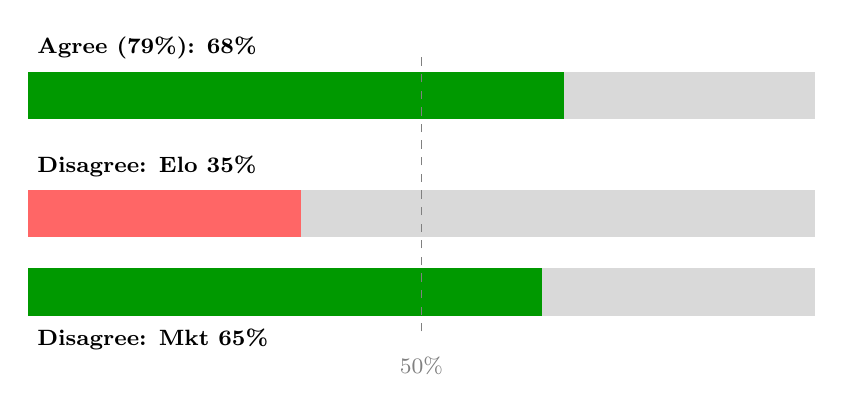
\begin{tikzpicture}
  % Agreement bar
  \fill[green!60!black] (0,2.2) rectangle (6.81,2.8);
  \fill[gray!30] (6.81,2.2) rectangle (10,2.8);
  \node[anchor=west] at (0,3.1) {\footnotesize \textbf{Agree (79\%): 68\%}};

  % Disagreement - Elo bar
  \fill[red!60] (0,0.7) rectangle (3.47,1.3);
  \fill[gray!30] (3.47,0.7) rectangle (10,1.3);
  \node[anchor=west] at (0,1.6) {\footnotesize \textbf{Disagree: Elo 35\%}};

  % Disagreement - Market bar
  \fill[green!60!black] (0,-0.3) rectangle (6.53,0.3);
  \fill[gray!30] (6.53,-0.3) rectangle (10,0.3);
  \node[anchor=west] at (0,-0.6) {\footnotesize \textbf{Disagree: Mkt 65\%}};

  % 50% line
  \draw[dashed, gray] (5,-.5) -- (5,3);
  \node[gray, anchor=north] at (5,-0.7) {\footnotesize 50\%};
\end{tikzpicture}%
}
\end{columns}
\end{frame}

% ================================================================
% SLIDE 6: Strong Favorites
% ================================================================
\begin{frame}[t]{Against Strong Favorites, Elo Is Wrong 84\% of the Time}

\begin{table}
\centering
\begin{tabular}{lrccc}
\toprule
Favorite Odds & N & Elo Acc. & Market Acc. & Avg Gap \\
\midrule
Heavy ($<$1.20) & 6 & \textcolor{badred}{16.7\%} & 83.3\% & 50pp \\
Strong (1.20--1.40) & 38 & \textcolor{badred}{15.8\%} & 84.2\% & 33pp \\
Moderate (1.40--1.60) & 80 & \textcolor{badred}{32.5\%} & 67.5\% & --- \\
Slight (1.60+) & 193 & 39.9\% & 60.1\% & --- \\
\bottomrule
\end{tabular}
\end{table}

\vspace{0.5em}
\textbf{Worst case:} Shelton vs Nishikori (French Open)\\
Market: 85\% Shelton \quad Elo: 23\% Shelton \quad Gap: \textbf{62pp} \quad Result: Shelton won

\vspace{0.5em}
\noindent Only \textbf{7 of 44} Elo contrarian picks against strong favorites were correct (16\%).
\end{frame}

% ================================================================
% SLIDE 7: Career Trajectory --- Root Cause
% ================================================================
\begin{frame}[t]{Root Cause: Elo Cannot Track Rapid Career Trajectory Changes}

\begin{columns}[T]
\column{0.48\textwidth}
\textbf{Underrated (Rising):}

\begin{table}
\centering
\footnotesize
\begin{tabular}{lccc}
\toprule
Player & 2022 & 2024 & Shift \\
\midrule
Etcheverry & 18\% & 52\% & \textcolor{goodgreen}{+34pp} \\
Struff & 24\% & 59\% & \textcolor{goodgreen}{+35pp} \\
Shelton & 50\% & 62\% & \textcolor{goodgreen}{+12pp} \\
\bottomrule
\end{tabular}
\end{table}

\vspace{0.5em}
These players improved sharply.\\
Elo still reflects their weaker past.\\
The market sees their current level.

\column{0.48\textwidth}
\textbf{Overrated (Declining):}

\begin{table}
\centering
\footnotesize
\begin{tabular}{lccc}
\toprule
Player & 2023 & 2024 & Shift \\
\midrule
Mannarino & 64\% & 33\% & \textcolor{badred}{--31pp} \\
Cachin & 42\% & 12\% & \textcolor{badred}{--30pp} \\
Nishikori & 67\% & 44\% & \textcolor{badred}{--23pp} \\
\bottomrule
\end{tabular}
\end{table}

\vspace{0.5em}
These players declined sharply.\\
Elo still reflects their stronger past.\\
The market prices in decline instantly.
\end{columns}

\vspace{0.5em}
\textbf{Mechanism:} Accumulated rating capital from hundreds of prior matches creates inertia that K=32 updates cannot overcome quickly enough.
\end{frame}

% ================================================================
% SLIDE 8: What's Missing
% ================================================================
\begin{frame}[t]{Three Outstanding Items from Previous Rounds}

\begin{table}
\centering
\begin{tabular}{p{4.0cm}ccp{4.5cm}}
\toprule
Item & Rounds & Status & Impact \\
\midrule
Calibration analysis & 5, 6 & \textcolor{badred}{Not done} & Distinguishes directional vs probabilistic errors \\
K-factor sensitivity & 3, 4, 5, 6 & \textcolor{badred}{Not done} & Directly tests trajectory lag fix \\
Statistical tests & 5, 6 & \textcolor{badred}{Not done} & Standard practice, model comparison \\
\bottomrule
\end{tabular}
\end{table}

\vspace{1em}
\noindent\textbf{K-factor sensitivity is the most actionable.} The trajectory analysis shows Elo has too much inertia. Higher K directly addresses this by weighting recent matches more. Testing K~$\in$~\{16,~24,~32,~48,~64\} on clean data requires a single backtest session with high diagnostic value.
\end{frame}

% ================================================================
% SLIDE 9: Proposed Fixes --- None Tested
% ================================================================
\begin{frame}[t]{Five Proposed Fixes Listed, Zero Tested}

\begin{table}
\centering
\footnotesize
\begin{tabular}{clp{3.5cm}cp{3.0cm}}
\toprule
\# & Fix & Mechanism & Effort & Status \\
\midrule
1 & Higher K-factor & More weight on recent results & Low & \textcolor{badred}{Untested} \\
2 & Time-decay & Older matches count less & Low & \textcolor{badred}{Untested} \\
3 & Form adjustment & Recent win rate multiplier & Medium & \textcolor{badred}{Untested} \\
4 & Refuse strong disagreements & Skip bets vs $<$1.40 favorites & Trivial & \textcolor{badred}{Untested} \\
5 & Hybrid model & Market prior + Elo adjustment & High & \textcolor{badred}{Untested} \\
\bottomrule
\end{tabular}
\end{table}

\vspace{0.5em}
\textbf{Recommendation:} Test fixes 1 and 4 first.

\begin{itemize}
  \item \textbf{Fix 1 (K-factor)}: Addresses root cause directly, one parameter change
  \item \textbf{Fix 4 (refuse disagreements)}: Trivial filter, eliminates 84\%-loss-rate bets, immediate ROI improvement
\end{itemize}
\end{frame}

% ================================================================
% SLIDE 10: Verdict and Recommendations
% ================================================================
\begin{frame}[t]{Verdict: Accept with Minor Revisions}

\textbf{Resolved:}
\begin{itemize}
  \item[\textcolor{goodgreen}{\checkmark}] Data leakage via \texttt{tourney\_date} mismatch --- properly fixed
  \item[\textcolor{goodgreen}{\checkmark}] Corrected results reported with leakage impact quantified
  \item[\textcolor{goodgreen}{\checkmark}] Root cause of Elo underperformance correctly identified
  \item[\textcolor{goodgreen}{\checkmark}] Honest conclusion: neither model beats the market
\end{itemize}

\vspace{0.5em}
\textbf{Minor revisions requested:}
\begin{enumerate}
  \item Run calibration analysis using existing \texttt{calibration\_summary()} function
  \item Test K-factor sensitivity: K $\in$ \{16, 24, 32, 48, 64\}
  \item Add binomial test on disagreement accuracy, McNemar test for model comparison
  \item Test ``refuse strong disagreements'' filter (skip bets vs $<$1.40 favorites)
  \item Update \texttt{model\_analysis.md} to distinguish pre- vs post-leakage numbers
\end{enumerate}
\end{frame}

\end{document}
